\section{Discussion}\label{sec:discussion}

Below, we reflect on the cost of training, re-training feasibility, confidence measure reliability, and final conclusions regarding the suitability of each learning algorithm. Training costs varied significantly across methods. Baseline classifiers using TF-IDF vectorization with 5,000 features took roughly one hour of CPU time each, alongside very high RAM usage of approximately 256 GB. In contrast, fine-tuning BERT took only about seven minutes on an 8x A100 GPU setup, which demonstrates remarkable efficiency once a pre-trained model is available—although training that model from scratch would be far more time-consuming. Retraining a fine-tuned BERT as new data arrives is therefore straightforward if adequate GPU resources and pre-trained checkpoints exist, while organizations with more limited resources might opt for traditional methods despite the high memory requirements.
\begin{comment}
    To assess how well the models’ predicted probabilities reflect actual risk, calibration plots were examined. Logistic Regression and SVM showed strong calibration, with only slight deviations at higher probability levels, whereas Naive Bayes exhibited poorer calibration, tending to understate its certainty. BERT’s curve formed an S-shape, suggesting that its probabilities are not well-aligned with real-world likelihoods, a shortcoming that could be addressed by employing post-training calibration methods such as temperature scaling. Still, BERT reached the highest performance (F1 score of 0.70 for the toxic class), making it a compelling choice where both speed and robustness are priorities. \cite{guo2017calibration}
\end{comment}


\begin{comment}
\begin{figure}[ht]
    \centering
    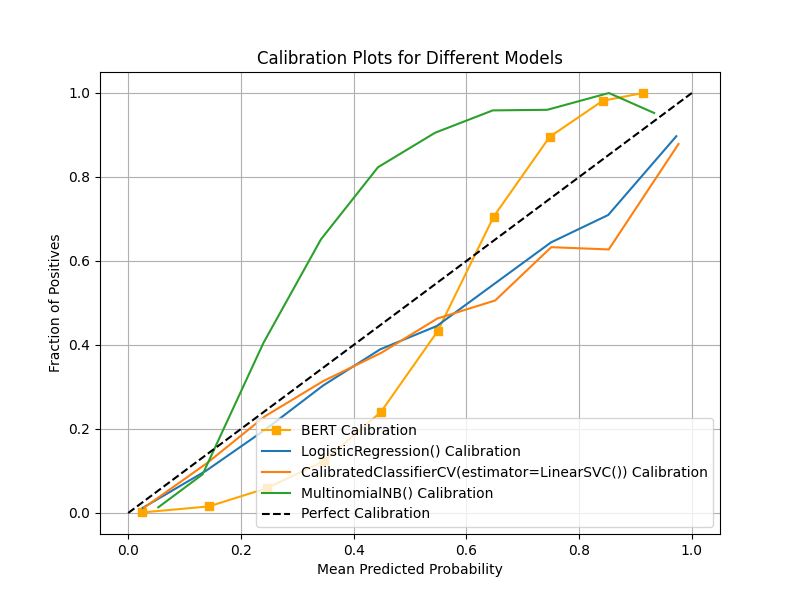
\includegraphics[width=0.7\textwidth]{./figures/calibration_comparison.png}
    \caption{Calibration plot for BERT and baseline models}
    \label{fig:calibration}
\end{figure}
\end{comment}

\noindent Traditional algorithms may be easier to train on CPUs and more accessible for quick iteration, though they can demand substantial RAM. Fine-tuned BERT, on the other hand, delivers stronger performance and can be retrained efficiently with adequate GPU support -- ideal for real-world scenarios requiring rapid updating. Adjusting the decision threshold can tailor the model’s behavior to specific guidelines or risk tolerances, and further improvements might come from adding more data (e.g., the Jigsaw Toxic Comment dataset) or transitioning to advanced transformer variants such as RoBERTa. Overall, BERT stands out as the most effective option when the necessary hardware is available, while simpler methods still offer a calibrated, albeit less powerful, alternative. \cite{Liu2019}